% !TeX root = ../Bachelorarbeit.tex
\chapter{Konzeption}
\section{Auswahl der Authentifizierungsverfahren}
Bei der Auswahl der Authentifizierungsverfahren musste vor allem berücksichtigt werden, inwiefern das Verfahren im Rahmen dieser Arbeit umsetzbar ist. Dies bezieht sich einerseits auf die Zeit, die es für die Implementation benötigt und andererseits auch auf die monetäre Machbarkeit. Es existieren für die Webauthentikation zum Beispiel ganz spezielle USB-Sticks von angesehenen Marken, die allerdings einige hunderte Euro kosten. Die Features die sie im Gegensatz zu einem ganz normalen USB-Stick (FIDO USB) liefern, beziehen sich dabei nur auf den Teil der Userverifikation. So besitzen einige USB-Sticks einen eingebauten Fingerabdrucksensor, ein Tastenfeld oder sogar zusätzliche Sicherheitssoftware auf den Massendatenträgern. Innerhalb dieser Arbeit sollte es allerdings um den Einsatz eines solchen Verfahrens für den Durchschnittsnutzer innerhalb von Unternehmen oder einen Casual Surfer gehen. Eine teure Anschaffung für die eigene Sicherheit erscheint dem Durchschnittsnutzer als nicht nötig.

Das Verfahren des Usernamen und des Passwortes wurde gewählt, weil es zum Verfassungszeitpunkt dieser Arbeit die Nutzer von Webseiten meist alleinig sichert. Die Loginverfahren größerer Dienste wie Microsoft Outlook, Google Mail und Facebook besitzen zwar schon seit Jahren die Möglichkeit der Authentifikation mit einem zweiten Faktor, doch das sind eher Ausnahmen. Ein Großteil der Internetpräsenzen ist sich entweder nicht der Risiken von Passwörtern für ihre Nutzer bewusst oder kann sich den Mehraufwand von neuen Verfahren nicht leisten. Gleichzeitig war es im Rahmen dieser Arbeit wichtig eine typische Implementation mit Username \& Passwort und ihren Scheinsicherheiten wie Hashes mit Salt und Pepper zu präsentieren. Es ist wichtig, den Ist-Zustand im heutigen Internet zu verstehen, um die Vorteile von neueren Methoden nachzuvollziehen.

Eine dieser neuen Methoden ist das zweite Verfahren. Nach dem Passwort ist das wohl der häufigste zweite Faktor den man findet. Apps wie der 'Google Authenticator' zählen mittlerweile als Synonym für das TOTP - Verfahren wie es im RFC beschrieben ist. Dies liegt unteranderem auch daran, dass die App tatsächlich die recht strikten Vorgaben aus dem RFC befolgt und nur minimale Unterschiede dazu aufweist. An dieser Stelle stellte sich eher die Frage ob HOTP oder TOTP in den Prototypen implementiert werden sollte. Es wurde sich für das TOTP - Verfahren entschieden, da es zwar den Mehraufwand der Synchronisation zwischen Zeit des Gerätes und des Servers benötigt doch dafür die Sicherheit der begrenzten Zeit bietet wie bereits erläutert.

Das dritte Verfahren, die 'Web Authentication', ist wohl das Erforschungswürdigste der drei Verfahren. Sie ist von allen drei Verfahren am seltensten auf Internetseiten vertreten und da stellt sich nach einer Analyse des Mehrwertes dieses Verfahrens die Frage nach dem Grund dafür. Im Gegensatz zu den anderen beiden Authentifikationsmethoden wurde Dieses nicht für den Prototypen ausgewählt, weil es so weit verbreitet und bereits genutzt wird sondern genau im Gegenteil: Es wurde gewählt, um mögliche Gründe zu suchen weshalb das Verfahren der Webauthn heutzutage kein Standard darzustellen scheint. Es muss untersucht werden ob es starke Nachteile Gegenüber der anderen Verfahren bietet, denn im Ansatz scheint es alle Nachteile des Passwortes auszumerzen.
\newpage

\section{Prototypenaufbau}

\begin{center}
    \center
    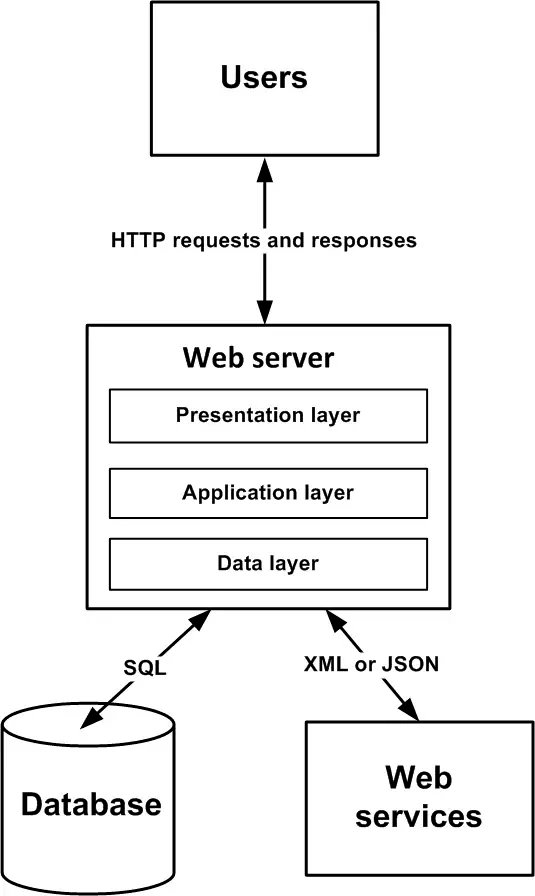
\includegraphics[width=10cm]{main-qimg-82af1fe49f85a31700d35570189a1fce.png}
\end{center} 

Das Ziel des Prototypen ist es, wie eingangs erwähnt, vorhandene Authentifizierungsverfahren abseits der klassischen UserID / Passwort Methode zu begutachten und dessen Schwächen aufzudecken. Daraus ergeben sich die typischen drei Komponenten von Drei-Tier-Client-Server Architekturen:

Ein Client, der Anfragen an die Applikation (das Backend bzw. den Server) sendet, welches die Daten dann in einer Datenbank mittels eines DBMS (Datenbankmanagementsystems) persistiert und verwaltet. Wie auch im Bild zur 3 Tier Architektur zu sehen, agiert der User auf dem Presentation Layer und stellt anfragen bzw. sendet JSON Objekte an den Server, der die entsprechenden Webservices liefert. Der Server speichert keine States, wodurch der Nutzer typischerweise mit jeder Anfrage alle benötigten Informationen liefern muss. Der Server liefert demnach lediglich die \ac{rest} Schnittstellen. Implementationsdetails und weitere Informationen zum Prototyp gibt es in folgenden Kapiteln.
